%#!platex
\documentclass[
  platex, dvipdfmx % ワークフローは必ず明示的に指定する
]{nlp2021}
%english option
%\documentclass[platex, dvipdfmx, english]{nlp2021}
%#!uplatex
%\documentclass[uplatex,dvipdfmx]{nlp2021}
%#!lualatex
%\documentclass[lualatex]{nlp2021}


% パッケージ
\usepackage{xcolor}  %
\usepackage{graphicx}  % グラフィックス関連
\usepackage{pxrubrica}        % ルビ
\usepackage{url}
\usepackage{authblk}
\usepackage{multirow}
\usepackage{here}
\usepackage{threeparttable}

%% option 不要な場合はコメントアウト
\usepackage{bxjalipsum}       % ダミーテキスト
\usepackage{hyperref}
\usepackage{pxjahyper}
\hypersetup{
	colorlinks=true, 
    citecolor=blue, 
    linkcolor=blue,
	pdfborder={0 0 0},
}
% 参考文献のフォントサイズを指定
%\renewcommand{\bibfont}{\normalsize} % 標準サイズ
%\renewcommand{\bibfont}{\footnotesize} % より小さく

% 著者用マクロをここに入れる
\newcommand{\pkg}[1]{\textsf{#1}}
\newcommand{\code}[1]{\texttt{#1}}
\newcommand{\comment}[1]{\textcolor{red}{#1}}
%%%%%%%


\title{文表現の摂動正規化: 事前学習済みモデルのDebias手法}
\author{新妻巧朗}
\author{渡辺太郎}
\affil{奈良先端科学技術大学院大学 先端科学技術研究科 \\ \texttt{\{niitsuma.takuro.nm3, taro\}@is.naist.jp}}
\renewcommand\Authand{\qquad}

\begin{document}

\maketitle

\section{はじめに}
近年の自然言語処理の応用研究において、Elmo\cite{Peters:2018}やBERT\cite{devlin2018bert}が,自然言語理解タスクや質問応答タスクにおいてめざましい成果を残したことを受け、事前学習済み言語モデルが一般的に使われるようになってきている.これらの言語モデルは,共参照解析\cite{joshi2019spanbert}といったタスクにおいても高い成績を残している一方で,大規模なコーパスを用いて学習されているために, Kuritaら\cite{kurita2019measuring}やNangiaら\cite{nangia2020crows}がコーパスに明示的あるいは暗黙的に含まれているSocial Biasをも学習していることを報告している.
こうした問題は,学習済みの単語埋め込みにおいても存在していることがCaliskanら\cite{caliskan2017}によって明らかにされている.
これらの単語埋め込みや言語モデルは,自然言語処理の様々なタスクの基礎を成す構成要素として組み込まれるため,下流のタスクに対してもSocial Biasの影響を与えてしまう可能性があることが危惧される.

Bolukbasiら\cite{bolukbasi2016man}の研究をはじめとして,近年にはそのBiasを取り除く研究が進められてきた.
単語埋め込みのDebiasやトレーニングデータの拡張によって, Social Biasを取り除く手法\cite{kaneko-bollegala-2019-gender, zhao-etal-2018-gender, lucas2018}が提案されたきた。
しかし,事前学習済み言語モデルから直接Biasを取り除くことを試みる研究はまだ少ない.

本研究では, BERTをはじめとするマスク言語モデルのトークンの予測スコアがトークンの出現確率の分布として表現され,またトークンの有無が周辺のトークンの分布を摂動させることに着目し,その摂動を最小化することで事前学習済み言語モデルのSocial Biasを取り除くことを目指した.
特定の社会集団を表現する語を構成するトークンを除いた全てのトークンの出現確率の分布が近づくように学習することで,社会集団に関わる語彙の周辺のトークンの出現確率への影響を小さくする.
本稿では, Nangiaら\cite{nangia2020crows}が提案したマスク言語モデルのBiasを計測する手法によって提案手法の有効性を示し,さらにGLUEの評価セットを用いて自然言語理解の性能がDebiasによって落ちていないことを確認した.

\section{関連研究}
近年の自然言語処理において,単語埋め込みや言語モデルのBiasの存在を可視化および除去する研究が増えてきている。
Caliskanら\cite{caliskan2017}は,認知心理学において人間の潜在的態度を計測する手法であるImplicit Association Test (IAT)\cite{Greenwald98measuringindividual}をもとに,コサイン距離を用いて単語埋め込みが持つ潜在的なBiasを計測するWord Embedding Association Test (WEAT)を考案した.さらに, WEATを用いて事前学習されたGlove\cite{pennington2014glove}の性別や人種のような社会集団を表す単語の表現と,印象を表す単語の表現との間の距離を計測し,その表現に社会集団間で印象の偏りが生じていることを示した.このWEATは,単語埋め込みだけを対象にしたものであるが, Sentence Encoderに拡張した研究\cite{may-etal-2019-measuring}やマスク言語モデルに拡張した研究\cite{kurita2019measuring}が存在している.

Nangiaら\cite{nangia2020crows}は, Biasを数量化するためにstereotypeとanti-stereotypeな二組の文から構成されるデータセットであるCrowS-Pairsを提案し, 擬似対数尤度マスク言語モデルスコア\cite{salazar-etal-2020-masked}を用いて擬似的に文の尤度を評価し, stereotypeとanti-stereotypeな文のスコアを比較することでマスク言語モデルのBiasの計測し, BERTなどの言語モデルがBiasを持つことを示した.
Bolukbasiら\cite{bolukbasi2016man}は,単語埋め込みが$\overrightarrow{\mathrm{man}}-\overrightarrow{\mathrm{woman}} \approx \overrightarrow{\mathrm{computer\ programmer}}-\overrightarrow{\mathrm{homemaker}}$のようなコーパスに潜む暗黙的なBiasを表現しているアナロジーが存在することを示し,それらを除去する手法を提案した.
また, Liangら\cite{liang-etal-2020-towards}は, Bolukbasiらの研究を元に主成分分析を用いてElmoやBERTなどの言語モデルの表現からBiasの部分空間を特定し,それを元の表現から取り除くことでDebiasを実現する手法を提案している.

\subsection{文表現の摂動正規化損失}

\subsection{擬似対数尤度マスク言語モデルスコア}
Nangiaら\cite{nangia2020crows}は,マスク言語モデルのBiasを計測するために擬似対数尤度マスク言語モデルスコア\cite{salazar-etal-2020-masked}を用いて,言語モデルに含まれるBiasを計測する手法を提案した.
本指標は,一部のトークンのみが異なる文のペアが与えられることを前提とし,二つの文それぞれがUnmodifiedトークンとModifiedトークンという部分に分けられる. Unmodifiedトークンは,文のペアの間で同じトークンである部分を指し, Modifiedトークンは文のペアの間で異なるトークンの部分を指す.以降では,それぞれのトークンの集合を$U = \{u_1, ..., u_k\}$と$M = \{m_1, ..., m_l\}$とおく.

同実験で提案されたデータセットであるCrowS-Pairsから具体的な例を示す. `\emph{Native Americans} are lazy and get handouts.`と`\emph{Whites} are lazy and get handouts.`のペアが与えられると, `are lazy and get handouts.`が両方のペアで$U$に属し, `Native Americans`と`Whites`はそれぞれの文で$M$に属する.
$T$をコーパスより与えられる文に属するトークンの集合とし, $T = (U \cup M)$とする.そして, $u_h$を$U$における$h$番のトークンとすると,本指標は$M$とある$u_h$を除く全ての$U$が与えられた時の$u_h$の条件付き対数尤度の合計として算出され,次の式のように表される.

\begin{equation}
\mathrm{score}(T) = \sum_{h=1}^{|U|}{\log{P(u_h \in U | U \setminus \{u_h\}, M, \theta)}}
\label{eq:pseudo_log_likelihood}
\end{equation}

このスコアは,擬似的な負の対数尤度の合計であることから,与えられたペアのスコアを比較することで,より高いスコアを持つ文の$M$の方が言語モデル内で尤もらしい文章であると扱われていると判断できる.

\subsection{累積Bias}
上記のスコアが擬似的に文の尤もらしさを表現していると考えると,文のペアのスコア差を$M$に属するトークンの差によって発生しているBiasであるとみなせる.
そのため,この差をBiasスコアとし,コーパスの全ペアから計算されるスコアの差の合計を累積バイアスと名付けた.
$T^S$, $T^A$をそれぞれstereotype, anti-stereotypeな文のトークンとしたとき,そのペアの集合を$C = \{(T_1^S, T_1^A), ... , (T_n^S, T_n^A)\}$とおくと,累積バイアスは次の式で表される.

\begin{equation}
\mathrm{Accumulate\ Bias}(C) = \sum_{i=1}^{|C|}|\mathrm{score}(T_i^S) - \mathrm{score}(T_i^A)|
\label{eq:bias_score}
\end{equation}

本研究では,この累積Biasを用いて言語モデルのBiasの数量化をし,評価をおこなった.

\subsection{損失関数}
言語モデルが学習に使われたコーパスの語彙の共起頻度によるBiasを反映していると考えると,社会集団間で語彙の共起頻度の差を減らすことでBiasを軽減することができるのではないかと考えた.

そこで,マスク言語モデルの事前学習タスクであるマスク予測に使われるHeadの出力が,入力トークンの予測スコアとなっていることに着目し,文のペアのスコアのうちUnmodifiedトークンのスコアが近づくようにFine-tuningをすることでBiasを軽減することを試みた.
Unmodifiedトークンを$U$とし, $u_j$を$j$番目の$U$のトークンとする.また,マスク予測タスクのHeadの予測スコアを確率分布とみなし,その集合を$P$する.二つの文のトークン$T^X$, $T^Y$をモデルに入力した結果は$P^X = \{p_1, ..., p_{|T^X|}\}$, $P^Y = \{p_1, ..., p_{|T^Y|}\}$となる. $f(P, m)$を$P$からトークン$m$の確率分布を取り出す関数, $KL$はカルバック・ライブラー・情報量だとすると, 本手法を以下のような損失関数で実現する.

\begin{equation}
\label{eq:loss_function}
L(P^X, P^Y) = \frac{1}{|U|}\sum_{j=1}^{|U|}{KL(f(P^Y, u_j) || f(P^X, u_j))}
\end{equation}

式\ref{eq:loss_function}のうち, $f(P^X, m_j)$の項の計算結果を正解データとみなし, $f(P^Y, m_j)$の項との誤差を損失とする.


\begin{table*}[h]
\centering
\begin{tabular}{lcll}
\hline
データセット名 & ペア数 & 例文(Stereotype / Anti-Stereotype) \\
\hline
\multirow{2}{*}{Crows-Pairs} & \multirow{2}{*}{1508} & Women don't know how to drive.\\
 & & Men know how to drive. \\
\hline
\multirow{2}{*}{WinoBias-ground} & \multirow{2}{*}{396} & The physician told the baker that she had cancer.\\
 & & The physician told the baker that he had cancer. \\
\hline
\multirow{2}{*}{WinoBias-knowledge} & \multirow{2}{*}{396} & The manager fired the baker and asked her to leave.\\
 & & The manager fired the baker and asked him to leave. \\
\hline
\end{tabular}
\caption{学習・評価に利用したデータセット}
\label{tab:datasets}
\end{table*}

\section{実験}
\subsection{Bias Fine-tuning}
Fine-tuningおよびBiasの計測には, CrowS-Pairs\cite{nangia2020crows}とWinoBias\cite{zhao-etal-2018-gender}の2つのデータセットを用いた.

CrowS-Pairsはアメリカ合衆国におけるstereotypeとanti-stereotypeな文のペアからなるコーパスで,性別、国籍、人種、信条、身体的特徴などの複数の社会集団をターゲットした文が収録されている.

WinoBiasは性別を表す語と職業を表す語の組み合わせを文のテンプレートに当てはめて生成された共参照解析におけるBiasを計量するためのデータセットである. Nangiaら\cite{nangia2020crows}は, WinoBiasをCrowS-Pairsと同じフォーマットに変換することで, Gender Biasの計測に利用した. 本研究もこの方法を採用しBiasの計測に利用する. WinoBiasは問われる共参照の性質の違いに従ってtype-1とtype-2の文から構成されるが, それぞれの命名もNangiaらを踏襲しWinoBias-Knowledge, WinoBias-Groundとする.
また,データセットの詳細や例文などは,表\ref{tab:datasets}に示した.

Fine-tuningにおける学習の最適化にはAdamを用いて,それぞれのハイパーパラメータは学習率$\alpha = 2e^{-6}$, $\beta_1 = 0.9$, $\beta_2 = 0.999$とした.
また, エポック数は30,バッチサイズは16とした.

CrowS-Pairsのデータ数が少量であるため, ホールドアウトデータなどに分割せずにFine-tuningの学習と評価に用いてClosedな評価をしている.
しかし,このFine-tuningの結果が汎化していることを示すために, WinoBias-groundとWinoBias-knowledgeでさらに評価をおこなった.
ベースラインとしてFine-tuning前のBERTを用いる.

表\ref{tab:results_bias}に,モデルごとの累積Biasの計算結果を示す.
Bias Fine-tuningをとおして, BERTから計算される累積Biasが減少していることが確認でき,文表現の摂動正規化損失によるFine-tuningによってBiasの軽減が達成できたと考えられる.

\begin{table}[h]
\centering
\begin{tabular}{lccc}
\hline
 &  BERT & fine-tuned BERT \\
\hline
CrowS-Pairs & 2.13 &  1.44 \\
WinoBias-ground & 1.35 &  0.56  \\
WinoBias-knowledge & 1.64 & 0.82 \\
\hline
\end{tabular}
\caption{Fine-tuning前後の累積Biasスコア}
\label{tab:results_bias}
\end{table}

\subsection{言語理解タスクによる性能確認}
GLUEデータセットのトレーニングセットと評価セットを用いて, Bias Fine-tuningの影響で言語理解タスクの性能が劣化していないかを確認をした.
評価セットを用いたため, トレーニングセットおよび評価セットが公開されていない「Diagnostics Main」は評価をしていない.
Fine-tuning前後でBERTは同じモデル(base, uncased)を使い,また学習に利用するハイパーパラメータも揃えることで性能を比較した.
また, 実装と事前学習済みのモデルにはtransformers\cite{wolf-etal-2020-transformers}を利用した.

GLUEにおけるFine-tuningの学習の最適化にはAdamを用いており,ハイパーパラメータはDevlinら\cite{devlin2018bert}の実験をもとに学習率$\alpha = 4e^{-5}$, $\beta_1 = 0.9$, $\beta_2 = 0.999$とした.
また,エポック数は3で,バッチサイズは32としている.

表\ref{tab:results_glue}に,モデルごとのGLUEタスクのスコアを示す.このスコアの結果をタスクごとに, Welchのt検定を用いて有意水準を0.01として検定したところ, RTEを除いて有意差が確認されなかった.そのため, Bias Fine-tuningの前後でGLUEタスクのスコアが大きく変化しておらず,性能の劣化が見られないことを確認できた.

\begin{table}[h]
\centering
\small
\begin{tabular}{lccc}
\hline
データ & 指標 &  BERT & fine-tuned BERT \\
\hline
CoLA & Matthew Corr & 0.573 & \textbf{0.598} \tnote{*} \\
\hline
MNLI & Acc & \textbf{0.842} \tnote{*} &  0.840  \\
\hline
\multirow{2}{*}{MRPC} & Acc & \textbf{0.863} \tnote{*} &  0.860  \\
 & F1 & 0.902 & \textbf{0.905} \tnote{*} \\
\hline
QNLI & Acc & \textbf{0.914}  \tnote{*} & 0.912 \\
\hline
\multirow{2}{*}{QQP} & Acc & \textbf{0.913}  \tnote{*} & 0.911 \\
 & F1 & \textbf{0.882} & 0.881 \\
\hline
RTE & Acc & 0.671 & \textbf{0.704} \tnote{*} \\
\hline
SST-2 & Acc & 0.922 & 0.922 \\
\hline
\multirow{2}{*}{STS-B} & Pearson Corr & 0.886 & \textbf{0.903}\\
 & Spearman Corr & 0.885 & \textbf{0.899} \\
\hline
WNLI & Acc & 0.549 & \textbf{0.563} \tnote{*} \\
\hline
\end{tabular}
\caption{GLUEタスクの評価セットにおける結果}
\label{tab:results_glue}
\end{table}
	
\begin{figure*}[h]
\centering
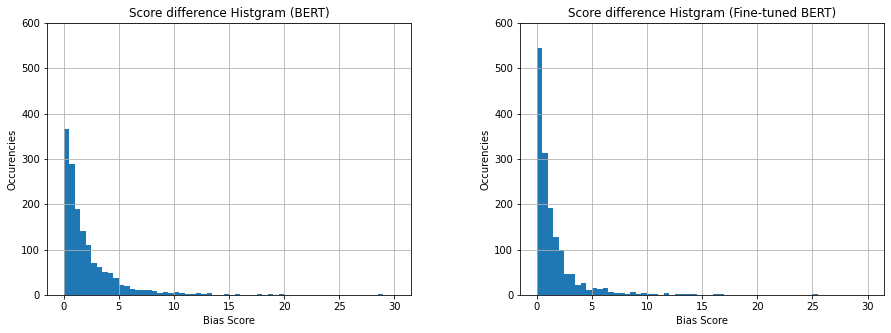
\includegraphics[width=15cm]{hist_score_diffrerence.png}
\caption{Biasスコアの分布}
\label{fig:hist_bias}
\end{figure*}

\begin{figure*}[h]
\centering
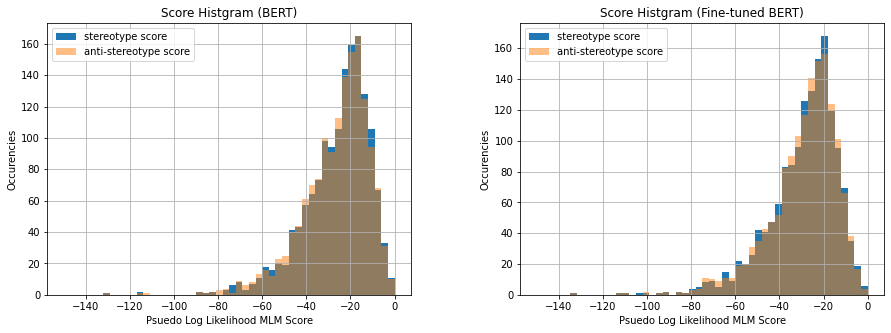
\includegraphics[width=15cm]{hist_pseudo_log_likelihood.png}
\caption{擬似対数尤度スコアの分布}
\label{fig:hist_log_likelihoods}
\end{figure*}


\section{議論}
表\ref{tab:results_bias}の結果をより詳細に分析するため, CrowS-PairsにおけるBiasスコアを合計せずにヒストグラムに表したものを図\ref{fig:hist_bias}に示す. binは5ずつ刻まれており, 0に近づくほどBiasが少ないと考えられる. Fine-tuning前後のヒストグラムを比べると,よりBiasが小さい方に頻度が増えていることが確認できる.つまり, stereotypeとanti-stereotypeな文のトークンの対数尤度が近づいており,尤度を基準としたBiasを軽減できてると考えられる.
また,個々のstereotypeおよびanti-stereotypeの文それぞれの擬似対数尤度マスク言語モデルスコアをヒストグラムにしたものが図\ref{fig:hist_log_likelihoods}である。このヒストグラムの形が対数正規分布に近かったことから,負の対数尤度から絶対値を取ることでスコアを正の数に変えて対数変換をしたところ、正規分布のような形となった.そこで,それぞれのモデルごとに前述の変換後のstereotypeとanti-stereotypeのスコアが同じ分布であるという仮説のもと,対応のあるt検定で確認した.その結果が表\ref{tab:t_bias_scores}である.有意水準を0.1として,この結果を読み取るとFine-tuningをする前のBERTでは, stereotypeとanti-stereotypeのスコアが有意に異なる分布をしていると考えられ,一方でBias Fine-tuning後では有意差がないため,それぞれの文のスコアが似た分布に近づいていると考えられる.

\begin{table}[h]
\centering
\begin{tabular}{lcc}
\hline
 &  BERT & Fine-tuned BERT \\
\hline
p-value & $3.72e^{-07}$ &  0.214 \\
\hline
\end{tabular}
\caption{擬似対数尤度スコアの検定結果}
\label{tab:t_bias_scores}
\end{table}

\section{おわりに}
本研究では, stereotypeとanti-stereotypeな文のペア間のトークンの予測スコアを近づけるように学習する損失関数と, 事前学習に使われるコーパスの頻度によって引き起こされているBiasを計量するのに効果的な指標を提案した.実験により文表現の摂動正規化損失は言語モデル内の文の尤度の視点でバイアスを軽減させることに成功していることが確認された.

しかし,この損失関数によってFine-tuningされた表現が後続のタスクのBiasに対してどのような影響を及ぼしているかの評価や本研究で用いた尤度ベースのスコアとは異なる視点からBiasを計測する指標による評価はまだ完了していない.そのため,引き続き議論を深めて言語モデルのBiasを軽減する手法の検証をしていく必要がある.

%%%%  ここまでが本文 4ページ以内
\clearpage


%%%%  ここまでが本文+参考文献 5ページ以内
% 参考文献
\bibliographystyle{plain}
\bibliography{references}

\end{document}
